\documentclass[final,hyperref={pdfpagelabels=false}]{beamer}
\usepackage{grffile}
\mode<presentation>{\usetheme{I6pd2}}
\usepackage[english]{babel}
\usepackage[latin1]{inputenc}
\usepackage{amsmath,amsthm, amssymb, latexsym}
\usepackage{subfig}
%\usepackage{times}\usefonttheme{professionalfonts}  % obsolete
%\usefonttheme[onlymath]{serif}
\boldmath
\usepackage[orientation=portrait,size=ua,scale=1.4,debug]{beamerposter}
\usepackage{ragged2e} 
\usepackage{bm}
% change list indention level
% \setdefaultleftmargin{3em}{}{}{}{}{}

%\usepackage{snapshot} % will write a .dep file with all dependencies, allows for easy bundling


\usepackage{array,booktabs,tabularx}
\newcolumntype{R}{>{\centering\arraybackslash}X} % right justified tabularx columns
\newcommand{\pphantom}{\textcolor{ta3aluminium}} % phantom introduces a vertical space in p formatted table columns??!!
\newcommand{\p}{\partial}
\newcommand{\bu}{\bm{u}}
\newcommand{\bv}{\bm{v}}
\newcommand{\imag}{\operatorname{Im}}

\listfiles

%%%%%%%%%%%%%%%%%%%%%%%%%%%%%%%%%%%%%%%%%%%%%%%%%%%%%%%%%%%%%%%%%%%%%%%%%%%%%%%%%%%%%%
\graphicspath{{figures/}}
 
\title{{\huge Vertical shear instability in the Solar Nebula}} 
\author{Min-Kai Lin and Andrew Youdin
  \\\vspace{1cm} \small{minkailin@email.arizona.edu, youdin@email.arizona.edu}}
\institute[UA]{Steward Observatory, 933 N Cherry Avenue,
  Tucson, AZ, 85721, USA}
%% \date[Sep. 8th, 2009]{Sep. 8th, 2009}

%%%%%%%%%%%%%%%%%%%%%%%%%%%%%%%%%%%%%%%%%%%%%%%%%%%%%%%%%%%%%%%%%%%%%%%%%%%%%%%%%%%%%%
\newlength{\columnheight}
\setlength{\columnheight}{105cm}
\setbeamertemplate{caption}{\centering\insertcaption\par}

%%%%%%%%%%%%%%%%%%%%%%%%%%%%%%%%%%%%%%%%%%%%%%%%%%%%%%%%%%%%%%%%%%%%%%%%%%%%%%%%%%%%%%
\begin{document}

\captionsetup[subfigure]{labelformat=empty}

\begin{frame}
  \begin{columns}
    % ---------------------------------------------------------%
    % Set up a column 
    \begin{column}{.49\textwidth}
      \begin{beamercolorbox}[center,wd=\textwidth]{postercolumn}
        \begin{minipage}[T]{.95\textwidth}  % tweaks the width, makes a new \textwidth
          \parbox[t][\columnheight]{\textwidth}{ % must be some better way to set the the height, width and textwidth simultaneously
            % Since all columns are the same length, it is all nice and tidy.  You have to get the height empirically
            % ---------------------------------------------------------%
            % fill each column with content            
            \begin{block}{{\Large Introduction}}
              \justifying
              {\large              
                {\bf
                  The Vertical Shear Instability (VSI) is a potential
                  route to purely hydrodynamic turbulence in cold
                  protoplanetary disks (PPDs). However, VSI requires rapid
                  cooling to be efficient.  We quantify the
                  thermodynamic dependence of the VSI using linear
                  theory, and apply our results to evaluate the
                  efficiency of the VSI in PPDs. We find VSI can operate
                  at $\sim 5$AU to $\sim 50$AU a typical PPD, with
                  characteristic growth times $\sim 30$ orbits. The
                  VSI is thus dynamically important in the outer disk,
                  with significant implications for mass accretion,
                  dust evolution, and thus planet formation. 
                }
              }
            \end{block}
            \vfill
            
            \begin{block}{{\Large Vertical shear and instability}}
              \justifying
              Astrophysical disks generally possess vertical
              shear, e.g. 
              \begin{align}
                r\frac{\p \Omega}{\p z} \simeq
                \frac{1}{2}\left(\frac{z}{H}\right)h q
                \Omega_\mathrm{Kep}\neq 0,
              \end{align}
              for a vertically isothermal disk. 
              \begin{itemize}
              \item $h \equiv H/r \ll 1$: disk aspect-ratio
              \item $q \equiv d \ln{T}/d\ln{r}$: radial temperature gradient
              \end{itemize}
              \textcolor{blue}{\emph{Instability due to $\p_z\Omega$?}}
              \begin{itemize}
              \item 
                Consider an exchange of two fluid elements, separated by 
                $(\Delta r,\Delta z)$ in space. Conservation
                of specific angular momentum imply a change in the
                kinetic energy by
                \begin{align}
                  \Delta E  \sim \Delta r^2 \left(\Omega^2 +
                    \frac{\Delta z}{\Delta r}\cdot r\frac{\p\Omega^2}{\p
                      z}\right). \label{simple}
                \end{align}
                \item Vertical shear is weak, \textcolor{blue}{{\bf BUT}}  
                \begin{align}
                  \Delta E &<  0 \quad \text{is possible if} \quad \left|\Delta
                    z\right|\gg 
                  |\Delta r|,\\
                  &\Rightarrow \quad \text{\textcolor{blue}{\bf
                      INSTABILITY!}}\notag 
                \end{align}
              \end{itemize}
            \end{block}
            \vfill
            \begin{block}{{\Large Super-fast cooling is needed!}}
              \justifying
              Eq. \ref{simple} assumes efficient cooling. 
              \textcolor{blue}{\emph{\bf{How fast does the disk need to
                  cool?}}}
            \begin{align}
               t_\mathrm{cool}\Omega_\mathrm{Kep} < \frac{h |q|}{(\gamma -
                1)} \equiv \beta_\mathrm{crit}\ll 1.   
            \end{align}
            \begin{itemize}
            \item Fast cooling is required to overcome strongly
              stabilizing effect of vertical buoyancy (adiabatic index
              $\gamma>1$).
            \item \textcolor{blue}{\emph{\bf{Stringent thermodynamic
                    requirement!}}}            \end{itemize} 
            \end{block}
            \vfill
            
            \begin{block}{\Large Linear theory}
              \justifying
              Growth rates from numerical solution to linearized fluid
              equations:\\
              \vspace{-1cm}
              \begin{figure}
                 \includegraphics[width=\linewidth]{figures/gcorr_compare_iso_maxrate_z5.ps}%\\
                 %\includegraphics[width=\linewidth]{figures/result2d_cool.ps}
               \end{figure}
               \vspace{-1cm}
               ($k_x$: radial wavenumber.)
               \begin{itemize}
               \item Rapid stabilization as cooling time is increased,
                 even by small amounts.
               \item \textcolor{blue}{\bf{$\beta<\beta_\mathrm{crit}$ 
                   is an excellent criteria for instability.}}
               \end{itemize}
            \end{block}
            \vfill
            % \begin{block}{{\Large Results in 2D}}
            %   \justifying
              

              
            % \end{block}
            % \vfill
          }
        \end{minipage}
      \end{beamercolorbox}
    \end{column}
    % ---------------------------------------------------------%
    % end the column
    
    % ---------------------------------------------------------%
    % Set up a column 
    \begin{column}{.49\textwidth}
      \begin{beamercolorbox}[center,wd=\textwidth]{postercolumn}
        \begin{minipage}[T]{.95\textwidth} % tweaks the width, makes a new \textwidth
          \parbox[t][\columnheight]{\textwidth}{
            \begin{block}{{\Large VSI in action}}
              \justifying
              \begin{figure}
                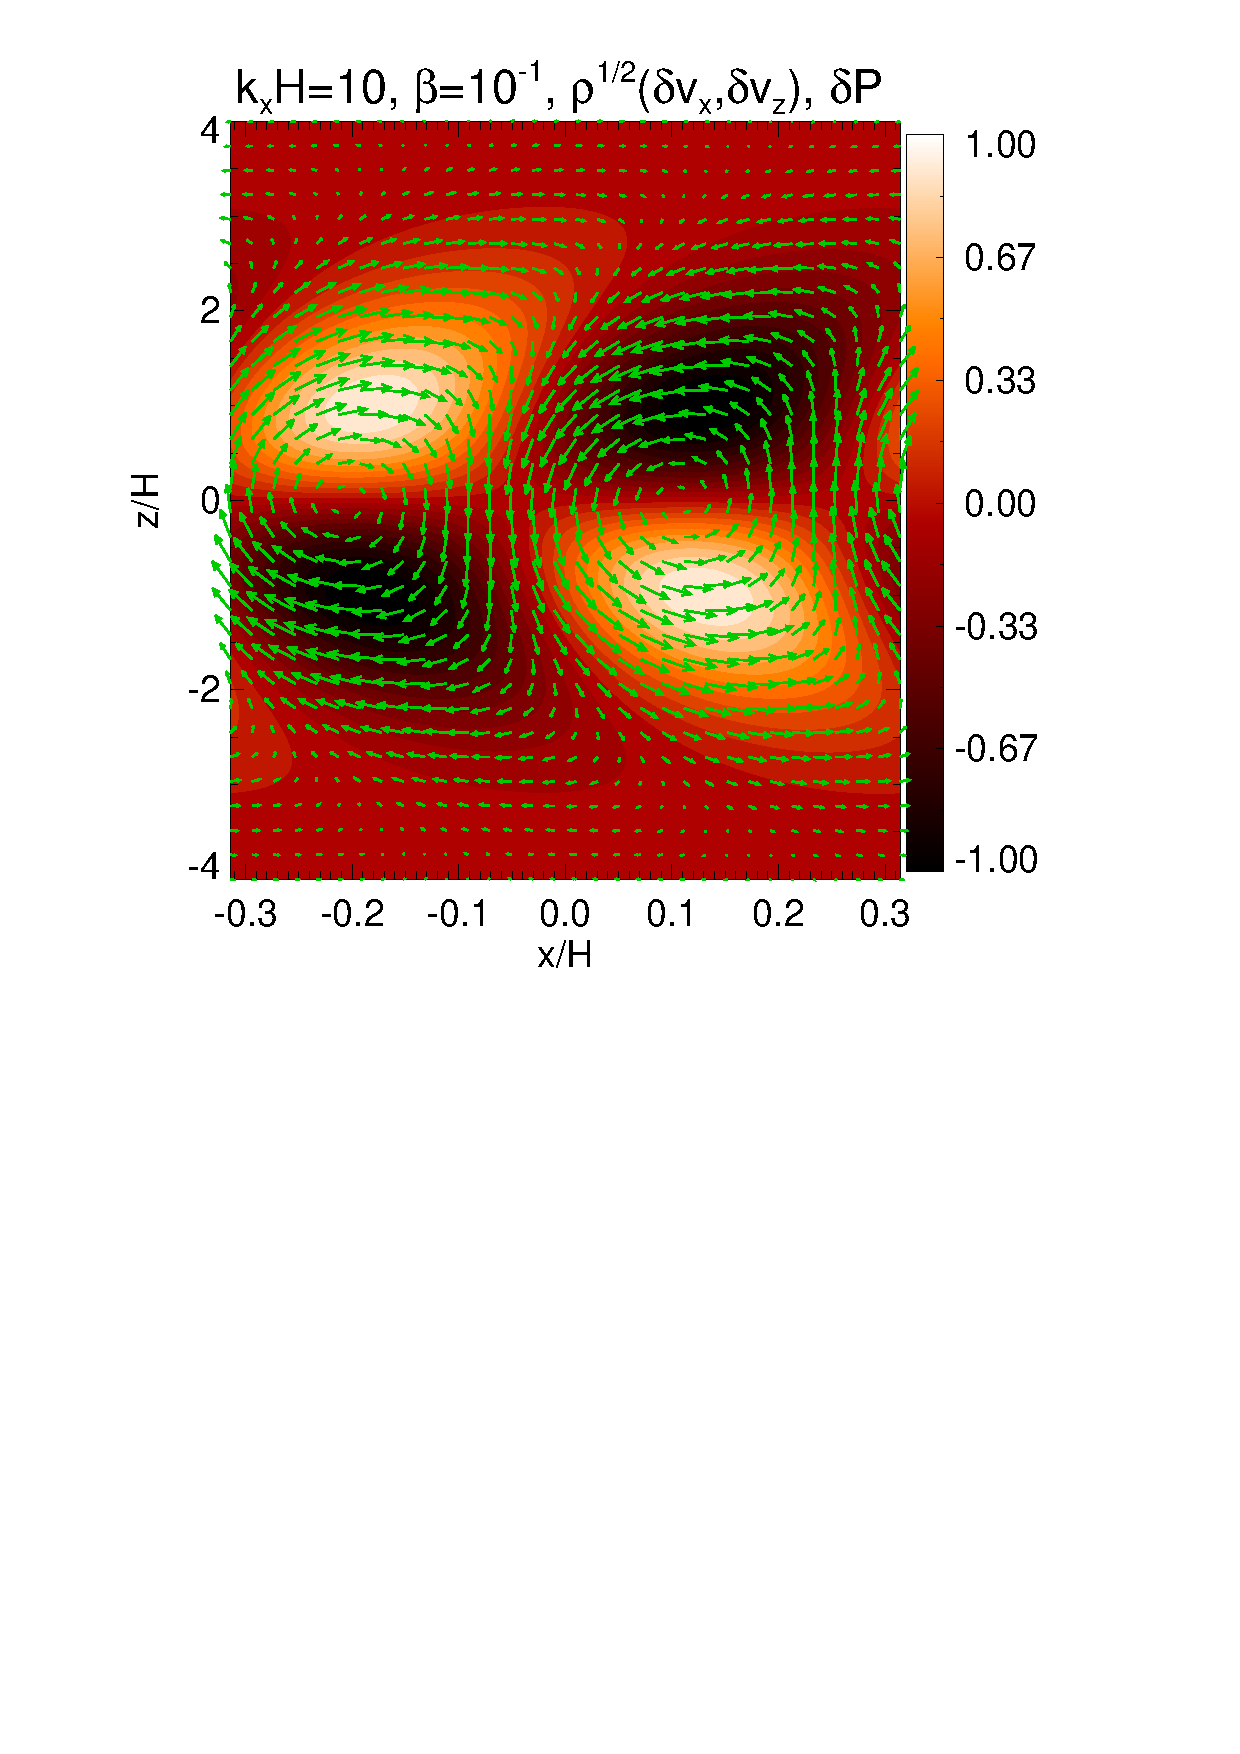
\includegraphics[width=\linewidth]{figures/result2d_cool}
              \end{figure}
              \end{block}
               
              \begin{block}{{\Large VSI in the Minimum Mass Solar Nebula}}
                \justifying
                Estimate actual cooling times in PPDs and compare with
                $\beta_\mathrm{crit}$:\\
                \vspace{-1cm}
                \begin{figure}
                  \includegraphics[width=\linewidth]{figures/bcrit_mmsn2d.ps}
                \end{figure}
                Numerical calculation of characteristic growth
                times:\\
                \vspace{-1cm}
                \begin{figure}
                  \includegraphics[width=\linewidth]{figures/eigen_compare_grow.ps}
                \end{figure}
                \begin{itemize}
                \item Efficient VSI in the outer disk at tens of AU. 
                \item VSI occurs on very small scales towards inner disk.
                \end{itemize}
              \end{block}
            \vfill
            % \begin{block}{\Large{Numerical model}}
            %   \justifying
            
            % \end{block}
            % \vfill

      
            \begin{block}{\Large{Summary}}
              \justifying
                  {\large              
                    {\bf
                      stuff
                    }
                  }
                \end{block}
              }
            \end{minipage}
          \end{beamercolorbox}
        \end{column}
        % ---------------------------------------------------------%
      % end the column
    \end{columns}
     % \begin{block}{\Large{Summary and discussion}}
     %           \justifying
     %            Large-scale spiral structures have been observed in
     %              the outer parts of transition disks. These could be
     %              due to unseen planets, but theoretical alternatives
     %              should be explored. We describe a 
     %              new but simple mechanism that can lead to the growth
     %              of one-armed spirals, or eccentric modes, in irradiated 
     %              astrophysical disks, which may be applicable to the outer
     %              parts of protoplanetary disks. We explain this new
     %              instability with linear density wave 
     %              theory, and confirm it through 2D and 3D
     %              hydrodynamic simulations. We find this mechanism can
     %              produce long-lived spiral structures. 
     %        \end{block}
    \vskip1ex
\end{frame}
\end{document}


%%%%%%%%%%%%%%%%%%%%%%%%%%%%%%%%%%%%%%%%%%%%%%%%%%%%%%%%%%%%%%%%%%%%%%%%%%%%%%%%%%%%%%%%%%%%%%%%%%%%
%%% Local Variables: 
%%% mode: latex
%%% TeX-PDF-mode: t
%%% End:
